\documentclass[landscape,a4paper]{article}
\usepackage[utf8]{inputenc}
\usepackage[T1]{fontenc}
\usepackage{tikz}
\usetikzlibrary{shapes,positioning,arrows,fit,calc,graphs,graphs.standard}
\usepackage[nosf]{kpfonts}
\usepackage[t1]{sourcesanspro}
\usepackage{multicol}
\usepackage{wrapfig}
\usepackage[top=0mm,bottom=1mm,left=0mm,right=1mm]{geometry}
\usepackage[framemethod=tikz]{mdframed}
\usepackage{microtype}
\usepackage{mathpartir}
\usepackage{graphicx}
\graphicspath{ {./images/} }
\usepackage{enumitem}% http://ctan.org/pkg/enumitem
\usepackage{amssymb} %% Definitions for math symbols.
\usepackage{amsmath} %% Definitions for math symbols.

\definecolor{myblue}{cmyk}{1,.72,0,.38}

\def\firstcircle{(0,0) circle (1.5cm)}
\def\secondcircle{(0:2cm) circle (1.5cm)}

\colorlet{circle edge}{myblue}
\colorlet{circle area}{myblue!5}

\tikzset{filled/.style={fill=circle area, draw=circle edge, thick},
    outline/.style={draw=circle edge, thick}}

\pgfdeclarelayer{background}
\pgfsetlayers{background,main}

\everymath\expandafter{\the\everymath \color{myblue}}
\everydisplay\expandafter{\the\everydisplay \color{myblue}}

\renewcommand{\baselinestretch}{.8}
\pagestyle{empty}

\global\mdfdefinestyle{header}{%
linecolor=gray,linewidth=1pt,%
leftmargin=0mm,rightmargin=0mm,skipbelow=0mm,skipabove=0mm,
}

\makeatletter % Author: https://tex.stackexchange.com/questions/218587/how-to-set-one-header-for-each-page-using-multicols
\renewcommand{\section}{\@startsection{section}{1}{0mm}%
                                {.2ex}%
                                {.2ex}%x
                                {\color{myblue}\sffamily\footnotesize\bfseries}}
\renewcommand{\subsection}{\@startsection{subsection}{1}{0mm}%
                                {.2ex}%
                                {.2ex}%x
                            {\color{red}\sffamily\bfseries}}
\makeatother
\setlength{\parindent}{0pt}

\begin{document}
\raggedright %%disable justification
\begin{multicols*}{3}
\fontsize{5.5pt}{4pt}\selectfont
\section*{OS Basics}
\begin{description}
  \item[OS] Intermediary b/w user \& HW, executes user programs. convenience, control and coordinate HW  (efficiency).
  \item[OS Services] user interface; prog execution; I/O operations; file-system manipulation; communication between Ps; error detection; res alloc; accounting – who uses how much of what; protection and security
  \item[Direct Memory access] Allow I/O devices to transfer data directly to/from main mem without involving CPU. (1 Interrupt per Data block) %NOTE: instead of 1 per byte (cpu cache)
  \item[Interrupt] request for processor to interrupt current executing code. Processor suspends activities, saves its state and starts executing/gives control to \textbf{Interrupt Service Routine}. \textbf{Interrupt Vector}: contains addresses of all (interrupt) service routines. OS is interrupt driven.
  \item[Trap, Exception] Software-generated interrupt. Caused by software error, system call, other process problems.
  \item[OS data structures] OS needs Lists, stacks queues, trees, maps
\end{description}

\subsection*{Multiprocessor (MP) Systems}
\begin{description}
\item[Advantages]Increased Throughput, Economy of scale, Reliability
  \item[Generic Approach] Each processor performs all (types of) tasks. OS shared among CPUs, each CPU has local private copy of OS data structures.
  \item[Asymmetric MP] Each processor is assigned a special task. Master CPU runs OS, other Slave CPUs run user processes.
  \item[Symmetric MP] Each processor performs all (types of) tasks. OS shared among CPUs. (Lock on OS)
  \item[Non-Uniform Memory Access (NUMA)] Interconnected CPUs each with private mem. They logically share one physical mem space.
  \item[Clustered Systems] Like MP, but multiple computers working together. Linked via some kind of network %NOTE: (e.g LAN).
\end{description}

\subsection*{OS Operations}
\begin{description}
    \item[Bootstrap Program] Initializes system, loads OS kernel and starts execution at power-up. (Stored in \textit{Firmware}). \hfill Degree of Multiprog = Nr. of Ps in mem.
  \item[Batch System, Multiprog.] schedule jobs so CPU always has one job to execute (keep job queue in mem).
  \item[Timesharing, Multitasking]  fast switching between jobs. interactivity for user(s). illusion of concurrency
  \item[Dual-Mode]User/Kernel. Distinguish whether system is running user or kernel code with a HW provided \textbf{Mode bit}. privileged instructions only run in kernel mode; sys. call $\rightarrow$ kernel mode. return $\rightarrow$ user mode. %NOTE: Timer (prevent $\infty$)
\end{description}

\fontsize{6pt}{4pt}\selectfont
\section*{OS Structures}

\subsection*{System Calls}
\begin{description}
    \item[System Call] Programming Interface to services provided by the OS written in high-level lang (C or C++), below user interface.
   \item[System Call Interface] Each system call associated with a number, Sys. Call interface maintains a table of those numbers, calls OS to execute and returns status and output.
   \item[Parameter passing] Either by passing parameters into registers (limited); or store them in a memory block and pass addresses in a register (unlimited length of parameter, limited amount of parameters); or push them onto stack (unlimited amount \& length)
  \item[Syscall types] File management, Device management, Information management, Communications, Protection

\end{description}

\subsection*{System Programs}
\begin{description}
  \item[System Program]Provides convenient environment for program development and execution. Often they are user interfaces to system calls
  \item[System Program Types] File management, Status information, Programming-language support, Program loading and execution, Communications, Background Services (daemons)
\end{description}

\subsection*{Application Programs}
\begin{description}
  \item[Application Programs]  designed to carry out a specific task other than one relating to the operation of the computer itself, typically to be used by end-users, e.g. web browsers.
\end{description}

\subsection{Creation of processes}
\begin{description}
  \item[1. Preprocessing] Reads c file, processes includes, expands macros, handles conditional compilation.
  \item[2. Compilation] Produces object code (.o), i.e. sequences of bytes, loadable into any memory location
  \item[3. Linking] Combines all object and library files into one executable file. Solves unresolved external references. Relocates machine addresses
  \item[Dynamic Linking] Conditionally linked libraries. Loads system libraries only once.
  \item[Static Linking] Necessary library functions are embedded directly in exe.
  \item[4. Loading] Shell/click creates P, invokes loader, loads exe to RAM. OS allocates memory, relocates memory addresses.
  \item[5. Execution] Program is a running P, CPU starts processing, upon completion returns status, releases resources, removed from memory



  \item[Executables across OSs] Apps compiled on one OS are not executable on other OSs. (differing system calls, binary formats, instruction sets application binary interface). Can be solved via interpreted langs, virtual machines, use of standard API with compiler generating binaries in OS specific language (e.g. POSIX)

\end{description}

\subsection{OS Structures}
\begin{description}
  \item[Monolithic Systems]Includes everything between user prog and hardware. + fast kernel communication, + little overhead, + easy interaction between OS modules, - difficult to change, maintain, - single failure can cause system crash, - gets complex fast.

  \item[Loadable Kernel Modules] Kernel can load independent modules such as device drivers when needed. Like layered Modules but more flexible as kernel can communicate directly. (Linux has this)
  \item[Layered Module Structure] OS is divided into layers, each built on top of lower layers. Each layer implements service and communicates only to lower level layers.
    \item[Microkernel Systems] Everything in user mode, except scheduling, virt. mem. and basic IPC in kernel mode. + easy to extend, + more reliable and secure, + easier to port, - more performance overhead of kernel and user space communication.
      \item[Hybrid Systems] Combines microkernel and monolitic approach to address performance, security, usability needs. OS partially in kernel and user mode e.g. Linux
\end{description}

% \vfill\null
% \columnbreak
\section*{Process Management}
\begin{description}
    \item[Process] Program loaded into mem, in execution.
  \item[Program] Passive entity stored on disk
  \item[Process states] new, ready, running, waiting, terminated
  \item[Process Control Block] Information about each P: P state, P number, PID, program counter, CPU registers, Mem.-management information (allocated mem for process), I/O status, CPU scheduling info (e.g. priority), Accounting info (e.g. CPU used)
  \item[Context Switch] When CPU switches to another P, save PCB of prev. P, load PCB of new P. (overhead)
\end{description}

\subsection*{Processes Layout}
\begin{tikzpicture}[remember picture,overlay]
    \node[xshift=76mm,yshift=5mm] at (current page.south west){%
    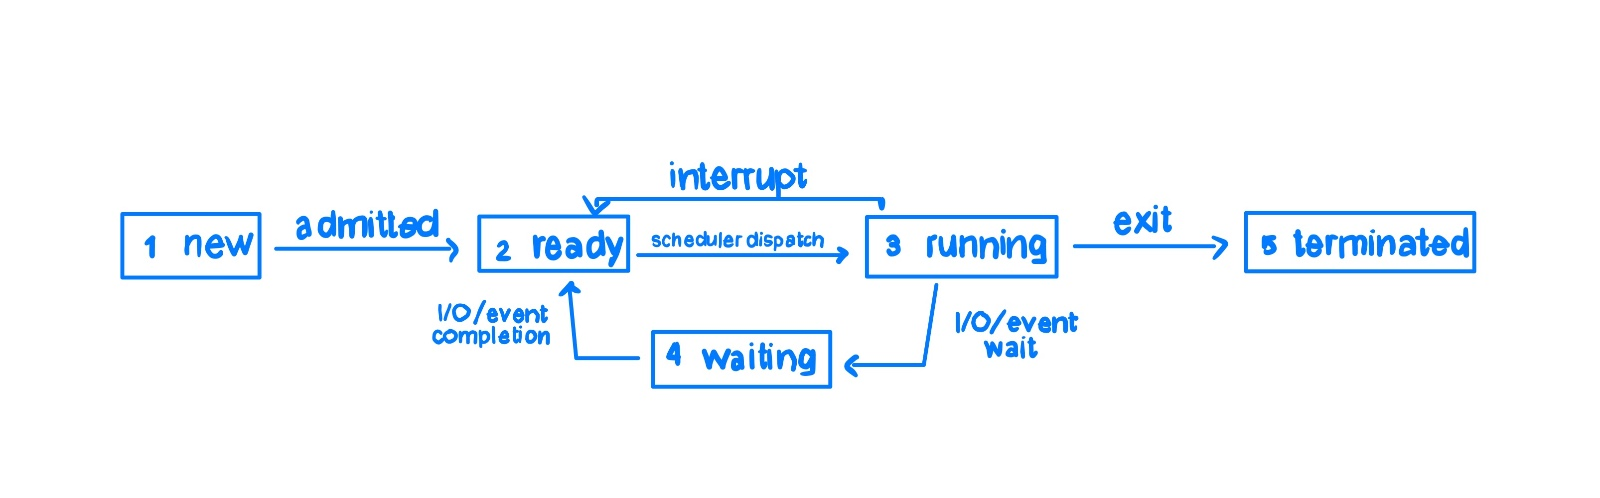
\includegraphics[width=55mm]{process_states.jpeg}};
\end{tikzpicture}
\begin{description}
  \item[Stack] temporary data: function parameters, return addresses, local variables
  \item[Heap] dynamically mem allocated during execution
  \item[data] Global variables
  \item[text] executable code
\end{description}

\subsection*{Operations on processes}
\begin{description}
  \item[Process creation]Parent P creates child (fork()) which can create own children → tree structure, every P has a unique identifier (PID). Either parent and child share all, a part or no resources.
  \item[Process termination] P's del themselves w/ exit(). Parent del child w/ abort(). Parent waits for child to end w/ wait(). child → \textbf{zombie} if child terminates before/w/o parent wait(), → \textbf{orphan} if parent terminates.
\end{description}

\subsection*{Interprocess communication}
\begin{description}
    \item[Cooperating P's](vs. Independent P's) execute concurrently, may be interrupted, share data. Need IPC
    \item[Shared Memory]Communication is under control of user P (not OS), P's share mem. space. Issue: \textbf{Producer-Consumer problem}: information to communicate stored in buffer. \textbf{unbounded:} no size limit, prod. can always produce, nice but unrealistic. \textbf{bounded:} fixed-size buffer. producer must wait if full.
  \item[Message passing] Communication controlled by OS, Messaging b/w P's w/out shared variables.\\
    \textbf{Communication Link}: \textit{Physical} (shared mem, HW bus, network). \textit{Logical}: direct/indirect, sync/async (blocking, non-blocking, rendez-vous),buffering (zero (sync r-v.)/bounded/unbounded capacity).
  \item[Direct Message passing] A link is established b/w P's. They must name each other explicitly (send(P,message), receive(Q,message)). Only one communication link. uni/bidirectional.
  \item[Indirect message passing] Messages are sent and received from mailboxes (i.e. ports). May share several communication links. uni/bidirectional.
  \item[Ordinary Pipe] Comm. b/w parent and child, cannot be accessed from outside the P that created it. Have a read end (fd[1]) and write end (fd[0]). Exists until P completion. (unidirectional)
  \item[Named Pipe, FIFO] Several P's can use pipe for communication. Exist until deleted. Appears as a file. (bidirectional: half/full duplex) %NOTE: duplex: travel one direction at the time or both at the same.
  \item[Socket] Endpoint of communication b/w machines, concatenation of IP and port. Data is sent via packets.
  \item[Remote Procedure Calls] abstract procedure (function) calls between Ps on networked systems. %NOTE: function can be invoked by P on another computer.
\end{description}

\section*{Scheduling}
\textbf{OS typically schedule threads and not processes}

\subsection*{Basic concepts}
\begin{description}
  \item[Scheduling queue] OS maintains a ready and wait (i.e. waiting for I/O or for child termination or for interrupt to be serviced) queue.
  \item[Short-term scheduler] Selects P which should be brought from ready queue to mem and allocates CPU time.
  \item[Long-term scheduler] Selects P which should be brought from job pool (possibly on disk) to ready queue
  \item[Dispatcher] Component, which gives control of CPU to P. Jobs: switching context, switching to user mode, jumping to proper location in program.
  \item[Starvation] A P has little to no CPU-time
  \item[Aging] The waiting time of a P is taken into account.
\end{description}

\subsection*{Scheduling Criteria}
\begin{description}
  \item[CPU utilization] $100 * cpu\_busy\_time / total\_time$
  \item[Throughput] $number\_of\_finished\_Ps_/time\_unit$
  \item[Turnaround time] Amount of time to complete a particular P $waiting\_time+exec\_time+i\_o\_time$
  \item[Waiting time] Amount of time a P is waiting in ready queue
  \item[Response time] time it takes from when a request was submitted until first response is produced by P. (e.g. web server handling request)
\end{description}

\subsection*{Scheduling Algorithms}
\begin{description}
  \item[First Come, First Served (FCFS)] Can lead to convoy effect, i.e. short P's waiting for long P's (starvation), which causes long avg. waiting time.
  \item[Shortest-Job-First (SJF)] Length of CPU-burst estimated with previous CPU-bursts of P. Is optimal, bc minimizes average waiting time.
  \item[Shortest-remaining-time-first (SRFT)] SJF with preemption, i.e. when P arrives with shorter burst-time than current running one, then current P is stopped and new P can run.
  \item[Priority scheduling (Prio)] Each P has fixed priority number. Lower number = higher priority. Higher priority first.
  \item[Round Robin (RR)] FCFS with preemption. each P can run for max fixed time q (\textbf{quantum time}). if q large $\leadsto$ FCFS , q small $\leadsto$ Context switching overhead.
  \item[Multilevel Queue Scheduling (MLQ)] Ready queue partitioned into separate ready queues. With each queue a priority number is associated. Each queue has own scheduling algorithm (e.g. foreground tasks with RR and background tasks with FCFS). A P is permanently in a given queue. If MQL preemptive $\leadsto$ starvation.
  \item[Multilevel Feedback Queue (MLFQ)] Like MLQ, but Ps can move between various queues (e.g. Ps with short burst-time or long waiting-time go to higher-priority queues). This avoids starvation. MLFQ is the most general algorithm, since it can be configured in many ways.
\end{description}

\subsection*{Thread Scheduling}
\begin{description}
  \item[Process Contention Scope (PCS)] Competition for CPU time is  among Ts within the same P. The user-level T library schedules, OS not involved in scheduling.
  \item[System Contention Scope (SCS)] Ts from different Ps, as well as Ts within the same P, compete for CPU time. OS is scheduling Ts. OS using one-to-one mapping model schedule Ts only using SCS.
\end{description}

\section*{Threads}
% \subsection*{}
\begin{description}
  \item[Threads] A basic unit of CPU utilization, executed within P.  Shared with P: code, data, files. Private: registers, stack, PC and own copy of T-local-storage (i.e. copy of static data)
  \item[Multithreaded benefits] responsiveness, resource sharing easier than with Ps, cheaper than P creation, lower overhead in context switching, scalability (even single P can take advantage)
  \item[Multiprocess benefits] being isolated, are better suited for tasks that require a  higher degree of separation and security.  \end{description}

\subsection*{Multicore Programming}
\begin{description}
  \item[Concurrency] More than one task making progress, tasks running out-of-order or in a partial order. (Software Parallelism)
  \item[Parallelism] Requires Concurrency and implies system can run more than one task simultaneously on multiple cores/nodes. (Hardware Parallelism)
  \item[Data Parallelism] distribute subsets of data across multiple cores, same operation on each core
  \item[Task Parallelism]  Tasks across  multiple cores, each task running unique operation(s).
  \item[Hybrid Parallelism] Combination of task \& data parallelism
  \item[Amdahl's Law] Speedup from N cores compared to 1 core w/ serial portion S: < 1 / (S + (1-S)/N
\end{description}

\subsection*{Multithreading Models}
\begin{description}
  \item[User threads (UT)] Ts in user space, which are not visible to kernel and managed without kernel support
  \item[Kernel Threads (KT)] Supported and managed by OS kernel
  \item[Many-to-One] Many UT mapped to one single KT. Not widely used, as one blocking UT blocks all UT and Ts don't run in parallel
  \item[One-to-One] Each UT maps to one KT (two-level-concurrency: Ts in both user and kernel space are concurrent). Number of Ts restricted due to causing overhead in kernel
  \item[Many-to-Many] Many UT multiplexed to many KT.OS creates as many KT as needed. Because of newer CPUs with many Ts, not that relevant anymore (starts to look like 1:1)
  \item[Two-level-Model] Many-to-Many with one single One-to-One exception (which needs guaranteed level of service).
\end{description}

\subsection*{Implicit Threading}
\begin{description}
  \item[Thread pool] Creation of a # of Ts that can be assigned to tasks, creation overhead is reduced.
  \item[Implicit Threading] Managing of Ts by frameworks. Programmer only has to identify tasks
\end{description}

\subsection*{Threading Issues}
\begin{description}
\item[Semantics of fork() \& exec()] if T invokes exec(), it replaces whole process with all Ts. fork() sometimes duplicates process with all Ts and sometimes only calling T.
  \item[Signal handling] (Signals are event based messages to a P) Problem: Where should a signal be delivered for a multithreaded P? Either same T is informed (sync), all Ts (async) or special signal T
  \item[Asynchronous cancellation] T terminates immediately
  \item[Deferred cancellation] T periodically checks if it should terminate (recommended)
  \item[Lightweight Process] A data structure between kernel and user Ts to manage appropriate number of kernel Ts allocated to app.
  \item[Scheduler activations] provide upcalls - a communication mechanism from the kernel to the app, to inform the app about events.
\end{description}

% \vfill\null
% \pagebreak
\section*{Synchronization}
Cooperating P's: execute concurrently, may be interrupted, share data. Maintain data consistency through Sequencing and Coordination.
% access: LAS or shared mem/message passing
\subsection*{Race Conditions}
Execution outcome dependent on order of concurrent access to shared data (ex: counter in prod-cons-prob, PID)
\begin{description}
        \item[solutions:] disabling interrupts (single core vs. multiprocessors (time-consuming), affects system clock)
            % TODO: Linux protection against race conditions: atomic variables, spinlocks, mutex locks
        \item[preemptive kernel:] P preempted in kernel mode, most common. more responsive, suitable for real-time programming
        \item [non-preemptive kernel:] uncommon, P blocks CPU
\end{description}

\subsection*{Critical Section Problem}
\begin{description}
    \item[critical section]is where a P accesses shared data (Structure: entry, critical, exit, remainder)
    \item[solution:]mutual exclusion (no 2 P in CS at the same time), progress (selection cannot be postponed indefinitely), bounded waiting (limit on waiting $\rightarrow$ Starvation)
    \item[Peterson's Solution]2 Ps, int turn, bool flag[2] shared, acquire \& lock, not guaranteed to work on modern computer architectures (requires atomic load/store, no instruction reordering)
    \item[Mutex Lock] acquire() and release() lock (atomic), bool available (binary), require busy waiting (spinlock, no context switch required)
    \item[Semaphores] integer variable, accessed through wait() and signal(). busy wait \\
        - \textbf{counting} (init to nr of resources available, decr. in wait) vs. \textbf{binary} semaphore (like mutex lock). \\
        -  \textbf{implementation with suspension and waiting queues} instead of busy waiting S suspends itself, each semaphore has associated waiting queue. signal() removes one P from list and awakens it.   %TODO: add code example
    \item[Monitors] high level form of P sync. (ADT, internal vars only acessible within procedures) \\
        - \textbf{condition variables} wait (suspends P) and signal (tells P to resume/condition could have changed) on condition var. \\
        - \textbf{mutex locks}: acquire and release are procedures in monitor
    \item[Priority Inversion] low-prio P holds lock needed by high-prio P. solution: \textbf{priority-inheritance protocol}: inherit higher priority until finished with resources
\end{description}

\subsection*{Bounded Buffer in Producer-Consumer-Problem}
Buffer with n slots, each can hold one item
\begin{description}
    \item[Semaphore Solution]3 S, init: mutex=1, full=0 (nr of fulls slots), empty=n.
    \item[- producer]wait(empty);wait(mutex); //produce signal(mutex);signal(full);
    \item[- consumer]wait(full);wait(mutex) //consume signal(mutex);signal(empty);
\end{description}

\subsection*{Dining Philosophers}
Allocate several resources among several Ps in a DL- and starvation-free manner. ex: 5 ph, 5 forks, 3 states (thinking, hungry, eating). Init: 1 data set (bowl of rise), chopstick[5], initialized to 1 (available).
\begin{description}
    \item[Simplest Solution] remove one ph %TODO: why?
    \item[Asymmetric Solution] odd/even pick up chopsticks asymmetrically
    \item[Monitor Solution]cond.var self[5], fun test(i) if hungry \& neighbours not eating $\rightarrow$ self[i].signal() \\
        - \textit{pickup(i)} set i to hungry, call test(i). if not eating afterwards, self[i].wait() \\
        - \textit{putdown(i)} set i to thinking, test left and right neighbour \\
        (starvation (requirement 3) still possible, can be solved by introducting time restriction)
\end{description}
    %TODO: S. 19 und 20 \subsection*{Synchronization within the Kernel}

\subsection*{POSIX Synchronization}
    \textbf{pthread.h} API is OS-independent (unix, macOS). provides mutex locks, named (accessible by multiple P's) and unnamed (need to be placed in shared mem) semaphores (include semaphore.h), condition variables (associated with a mutex lock).
    %TODO: S. 26 OpenMP

\subsection*{Deadlocks}
\begin{description}
    \item[Deadlock]2 or more P's are waiting indefinitely for an event that can be caused only by one of the waiting Ps. 4 conditions: \textbf{Mut. Ex.}, \textbf{Hold and wait} P that holds min. 1 res waits for another res. \textbf{No preemption} res can only be released voluntarily by P holding it. \textbf{Circular Wait} Cycle in res-alloc graph
    \item[Resource-Allocation Graph] Cycle necessary \& sufficient condition (possibility if several instances) %TODO: add picture
    \item[Handling Deadlocks]\textbf{1}. Ensure that sys never enters DL: DL prevention/avoidance ( allow res-alloc only if no DL could happen) \textbf{2}. Allow DL, detect and recover from it. \textbf{3}. Ignore DLs (approach of most OS, user is responsible)
    \item[Deadlock Prevention]: Eliminate at least 1 cond (only D4 practical to eliminate) \\
    \textbf{D1:} Use shareable res (e.g. read-only files) \textbf{D2:} Only req. res if P doesn’t hold other res (problem: low res util/ starvation) \textbf{D3:} (if res not available: first free all, restart if all needed res can be acquired at once) \textbf{D4:} Impose total ordering on all res-types. Requests allowed only in increasing order of enumeration.
    \item[Livelock] P or T continuosly attempts an action that fails. (failure to succeed) %TODO: nochmal anschauen
    %TODO: insert example of deadlock with mutex locks
\end{description}

% starvation

\section*{Memory Management}
\subsection*{Main Memory}
MM is the only storage the CPU can access directly. \textbf{Speed:} CPU Registers > Cache > Main Memory.
\begin{description}
    % Main Memory Partitions: resident OS in high PA, user Ps usually in low pa
    \item[Base and limit registers] smallest legal mem. address + size. Define \textbf{Logical Address Space (LAS)} of a P (set of all LA's). P can only access mem inside LAS (otherwise trap $\rightarrow$ fatal error). Only OS can access all registers/mem. \\
    \item[Logical Address / Virtual Address] generated by CPU. visible to user. editable \\
    \item[Physical Address] only seen by Mem. Unit. does not change. \textbf{PAS} set of  all PAs correspoding to LAS \\
    \item[Address Binding] mapping instructions and data to mem addresses. 3 schemes/stages: (in red) \\
    %TODO: 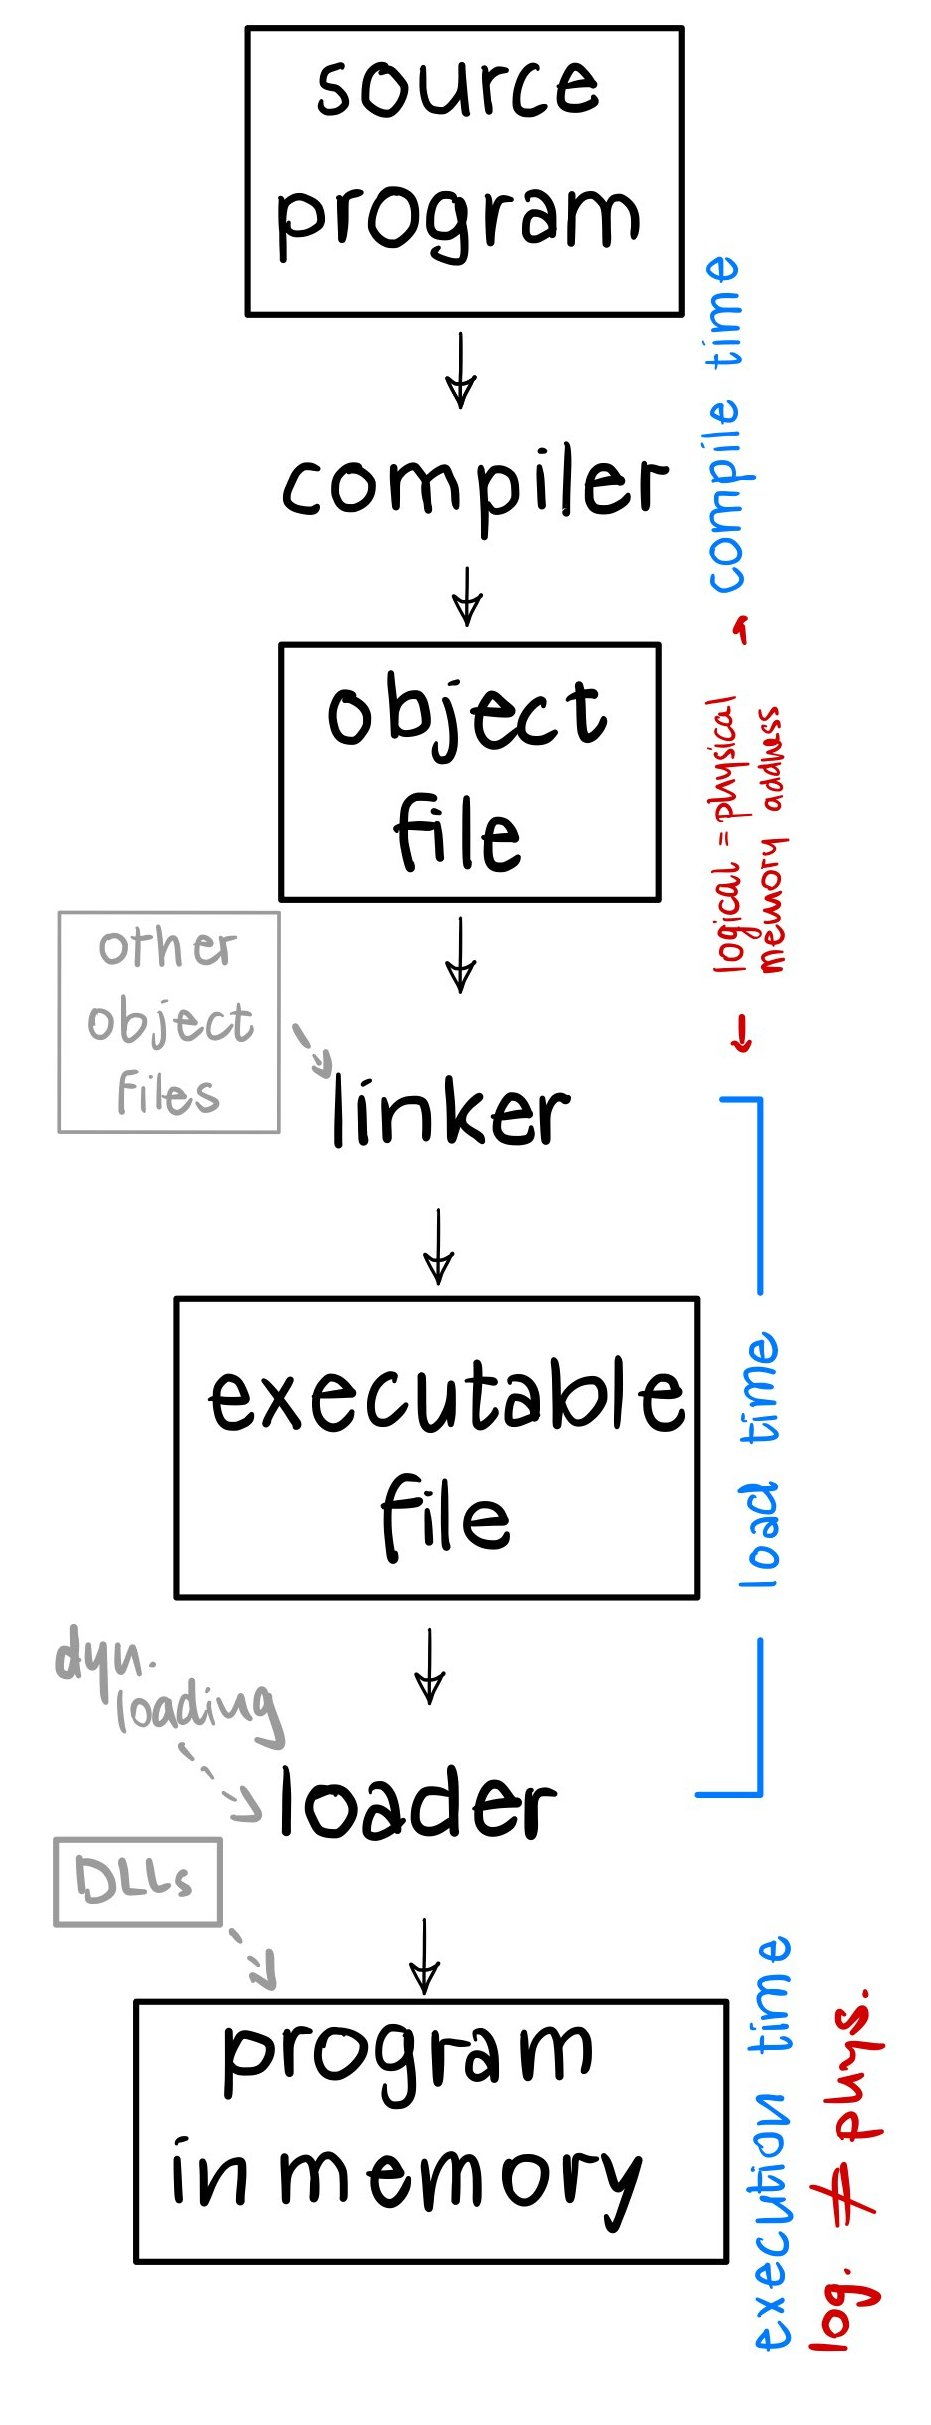
\includegraphics[width=\linewidth]{05_mem.jpg}
    \item[Memory Management Unit MMU] HW device, maps LA to PA during execution. $\rightarrow$ mapping methods (relocation register, contiguous paging) \\
    \item[Dynamic Loading]: routine not loaded in mem until called. all routines kept on disk. no special os support needed \textbf{Static Linking}: Libraries and program code combined by loader. \textbf{Dynamic Linking} happens during execution. useful for shared libraries (standard C lib.) DLL: dynamically linked libraries. \\
    \item[Contiguous Memory Allocation] each P is contained in a single section of mem that is contiguous to the section containing the next P. \textbf{Memory Protection:} through usage of Relocation \& limit registers. degree of multiprog. limited by nr of partitions. \\
    \item[Dynamic Storage Allocation]: OS maintains list of allocated and free partitions (\textbf{Holes}). First-fit (fastest), Best-fit (eq. to ff in storage-utilization, produces smallest leftover-hole), worst-fit (produces largest leftover hole) \\
    \item[Internal Fragmentation]: physical mem organized into fixed-size blocks. happens if allocated mem larger than requested mem (internal to partition). \\
    \item[External Fragmentation]: Total Mem Space for requests exists, but is not contiguous. 50\% rule: 1/3 unusable. \textbf{Solutions} \textit{Compaction}: moving data, can be expensive, only possible with dynamic address relocation (during ex. time) \textit{Noncontinguous Allocation}: Strategy used in Paging \\
    \item[Paging] PA can be noncontiguous, mem for P allocated wherever possible (no ex. fragmentation, but some internal $\rightarrow$ smaller pages eq. less int. frag but move overhead in page table). Physical mem is divided into fixed-size blocks called \textbf{frames}. Logical mem divided into same-sized blocks called \textbf{pages}.\\
    \item[Adress-Translation]: page number and page offset in the per-P page table
    % 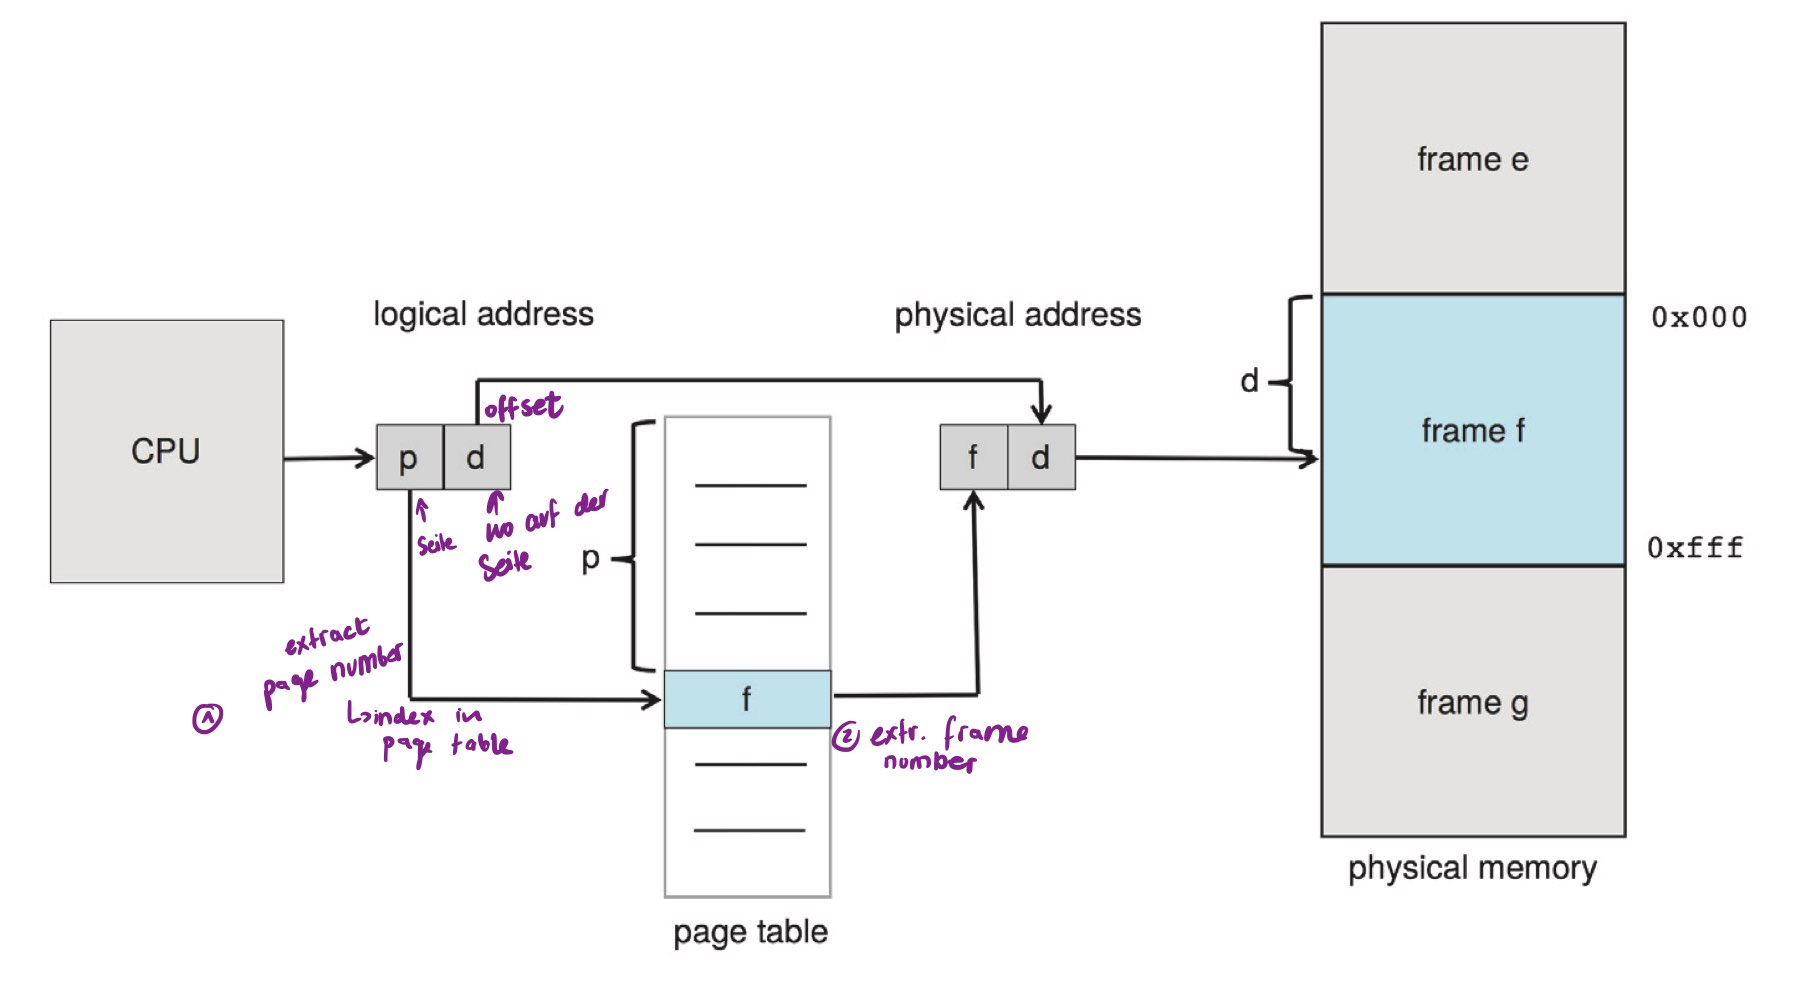
\includegraphics[width=0.4\linewidth]{05_paging.jpg} %TODO: modify image to include TLB
    \item[] OS keeps copy of each per-P page table + maintains frame table (for each physical frame)
    \item[Hardware Implementation]: per-P page table kept in main mem. \textbf{PTBR} page-table base register (pointers) \& \textbf{PTLR} page-table length register (size of page table)
    \item[Translation Lookaside Buffer TLB]: associative mem. hw cache for page table. (page nr, frame)
    % TODO: replacement policies: round-robin, LRU, random. key kernel code can be wired down for permanent fast access
    \item[Memory Protection] protection bit (read-only, read-write) or valid-invalid bit (attached to each entry in the page table. indicates if legal (in LAS) or not)
    \item[Shared Pages]: reentrant (unchanging) code shared among Ps. ex: Standard C libary
    \item[Structure of the Page Table] \\
    \item[Hierarchical Page Table]: ex: two-level page table, page the page table. (forwa[d mapping) \\
    \item[Swapping]: moving P temporarily out of mem to a \textit{backing store} and brought back for continued execution. (P roll out, roll in). system maintains ready queue. $\rightarrow$ transfer time too high, not used in modern OS  \\
    %TODO: hashed page tables, inverted page tables (if addresses expand beyond 32bits)
    \item[Swapping with Paging]: pages of a P instead of whole P swapped. (page in, page out)
\end{description}

\subsection*{Virtual Memory}
Abstracts main memory into an extremely large, uniform array of storage (LAS > PAS). Allows execution of partially-loaded programs. (more programs can run at the same time, increased CPU utilization \& throughput, no increase in reponse/turnaround time, less I/O needed to swap processes )
\begin{description}
    \item[Demand Paging]: bring page into memory only when it is needed (when \textit{page fault} occurs). \textbf{HW Support}: Valid-Invalid Bit (v: legal & memory resident, i: not valid or not-in-memory). PPP-table, Secondary Memory with swap space, Instruction restart. \textbf{Pure demand paging}: extreme case where process starts with no pages in memory.
    \item[Copy-on-Write]parent and child P initially share the same pages in memory. modifiable pages marked as CoW, copied only if page changes.
    \item[Free-Frame List]Pool of zero-fill-on demand pages (frame cleared with 0's, before released to P). \\ %TODO: pages/frames ?
    $\rightarrow$ no free frame? \textbf{Page Replacement}: select victim frame (requires 2 page transfers: page-out victim and page-in desired page, overhead can be reduced by using modify/dirty bit) %Page replacement and Demand paging complete separation between physical and virtual memory
    \item[Page Replacement Algorithms] Decide which pages are replaced, reduce page-fault rate (nr of page faults minimally decreases with more frames). \textbf{FIFO}: oldest page replaced (doesn't say anything about usage of page), suffers from \textbf{Belady's anomaly}: Adding more frames can increase the number of page faults. \textbf{Optimal algorithm}: Replace the page that will not be used for the longest period of time. not possible in practice bc it  requires future knowledge. \textbf{LRU}: least recently used, replace page that has not been used the longest time.
    \item[Allocation of Frames]How many frames are given to each process? \textbf{Fixed Allocation}: equal or proportional to process size. \textbf{Priority Allocation}: proportional to priority (sometimes &size). \\
        \textbf{Replacement}: select replacement frame from the set of all frames (\textbf{global}, no keeping track of which P replaced pages belong to) vs. own set of frames (\textbf{local}).
        %global: P execution time can vary greatly, greater throughput (more common). local: more consistent per-process performance, but possibly underutilized memory TODO: Numa S. 44
    \item[Thrashing] P does not have enough frames to support the pages int he working set $\rightarrow$ high page-fault rate $\rightarrow$ low CPU utilization $\rightarrow$ OS increases multiprog (with global r. alg.) $\rightarrow$ more thrashing
    \begin{itemize}
        \item \textbf{Locality}: set of pages that are actively used together by a P.
        \item \textbf{Locality Model}: all programs will exhibit a basic patterned memory reference structure, page-faults occure only when it changes locality (of memory-reference). Thrashing occurs when sum of locality sizes > total Phys. Memory, can be limited by using local replacement algorithm, or simply providing enough memory.
    \end{itemize} %TODO: Working Set Model, ev. OS Examples ?
\end{description}

\fontsize{5.5pt}{4pt}\selectfont
\section*{File Systems}
\begin{description}
    \item[File System]mechanism for storing and accessing data and programs. \textbf{Files} contain data, \textbf{Directory structure} organizes and stores information about files.
    \item[File]\textbf{OS View}  named collection of related info (\textbf{OS View}). smallest unit to store info in sec. storage (\textbf{User View})

\end{description}

\fontsize{6pt}{4pt}\selectfont
\section*{Virtualization}
Abstract the HW of a single computer (CPU, RAM, Storage) into different execution environments. \\
\begin{description}[labelsep=0pt]
    \item[] \textbf{Host} underlying HW system. \textbf{Hypervisor/VM Manager} provides interface identical to host. \textbf{Guest}
    \item[History] \hspace{2pt} \textbf{Multicomputer Model} Each computer provides different service (+ reliable, isolation (sandboxing), - Maintenance, Scalability) \textbf{Virtualization} overcomes limitations. run multiple OS on one machine, Prototyping, support checkpointing and VM Migration. %TODO: checkpointing, vm migration ?
\end{description}
\begin{description}
    \item[Implementation of Hypervisors]:
        \begin{itemize}[label={}, labelsep=0pt]
        \item \textbf{Type 0}: HW-based solutions, support VM creation and management through \textit{firmware} (VMM itself is encoded in firmware and loaded at boot-time) %limited features bc HW
        \item \textbf{Type 1}: OS-like software or OS's, VMM runs in kernel mode (ex: Windows HyperV, ..), common in data centers, live migrations (balance performance, efficiency), snapshots, cloning.
        \item \textbf{Type 2}: applications that run on standard OS (VMM is a process), limited hw feature exploitation. (ex: VirtualBox) %TODO: evt. add comparison picture type 1 & type 2
        \item \textbf{Emulators}: allow apps written in one system architecture to run on different system arch.
        \item \textbf{Programming Environment Virtualization}: no virtualization of real HW, but creation of optimized virtual system (ex: .NET, JVM)
        \item \textbf{Paravirtualization}: avoids causing traps by modifying guest OS source code
    \end{itemize}
\end{description}
\subsection*{Building Blocks}
Exact Duplicate of HW difficult to provide (esp. with dual-mode operation (kernel/user mode))
\begin{description}
    \item[VCPU]Virtual CPU to represent the state of CPU per guest (as guest believes it to be).  %does not execute code, information from VCPU used during context-switches
    \item[Trap-and-emulate] virtual user mode and virtual kernel mode (guest runs in physical user mode). privileged instruction (ex. sys calls) $\rightarrow$ trap to VMM $\rightarrow$ VMM emulates action $\rightarrow$ return control to guest (kernel mode slower $\rightarrow$ hw support)
    \item[Binary Translation] For CPUs that do not cleanly differentiate privileged instructions. VCPU in user mode $\rightarrow$  run instructions natively. VCPU in kernel mode $\rightarrow$ inspect next few instructions, \textit{Special Instructions} are translated and executed.
    \item[Hardware Support]enables more stable, faster and feature rich virtualization. more CPU modes, hw support for Nested Page Tables, DMA, interrupts (ex: Intel VT-x, AMD: AMD-V)
\end{description}
\subsection*{Virtualization and OS Components}
How do VMMs provide core OS-functions ?
\begin{description}
    \item[CPU Scheduling]VMM acts like multiprocessor system, schedules phys. CPU to VCPUs (using algos). %2 scenarios: enough CPUs, Overcommited, can cause clock drift
    \item[Overcommitment]Guests are configured to use more CPUs/Memory than physically available.
    \item[Memory Management] More Users of Memory $\rightarrow$ more pressure. Overcommitment common. VMM maintains \textbf{Nested Page Table} that translates guest page to real page table. (optimize without user knowing, own page-replacement-algos)
    \item[Storage Management] need to provide boot disk \& general data access. (support many guests, so partitioning not sufficient)
        \begin{itemize}[label={}, labelsep=0pt]
            \item \textbf{Type 0}: store guest root disks \&config as disk image in FS provided by VMM
            \item \textbf{Type 1}: store as files in FS provided by host OS %TODO: evt. mehr infos (S. 27)
        \end{itemize}
    \item[Live Migration]copy running guest to another system. (interesting: MAC must be movable (network). Limitations: Disks cannot be moved. (solve: make remote) \\
    src connects to T(target) $\rightarrow$ T creates guest $\rightarrow$ send readonly pages $\rightarrow$ send read-write pages (clean) $\rightarrow$ send dirty pages (modified, repeatedly) $\rightarrow$ send VCPU's final state and start T $\rightarrow$ terminate source
\end{description}
\subsection*{Containerization}
\begin{description}
    \item[Application Containment]run applications in isolated environment. create virtual layer between OS and applications. Each zone has own applications, Network Stack, Addresses, ... CPU and RAM divided between zones.
    \item[Containers]Standardized Packaging for Software and its Dependencies. Multiple instances, Portable, Isolated (Security), Less Ressource Usage, Quick Startup, Fast(er) Live Migration, Consistent and Reliable Running Env.
    \item[Docker]: %Controlled Namespace for Host Process Environments
        \begin{itemize}[label={}, labelsep=0pt]
            \item \textbf{Image}: represents full applications (store app)
            \item \textbf{Container}: application service location and execution (run app)
            \item \textbf{Engine}ju: Creates, ships and runs Docker containers
            \item \textbf{Registry Service (Docker Hub)}: CLoud or server-based storage \& distribution service for images
            \item \textbf{Dockerfile}: Commands that build Image layer-by-layer (ex: alpine $\rightarrow$ python $\rightarrow$ ..)
        \end{itemize}
        %TODO: add comparison image VMs vs. Containers
\end{description}

\section*{Parallelization Steps}

\section*{OpenMP}

\end{multicols*}
\end{document}
